\section{Introduction}

Dans un environnement où les systèmes d'information deviennent de plus en plus complexes et interconnectés, la gestion manuelle des infrastructures techniques pose de nombreux défis. Les entreprises doivent faire face à des exigences croissantes en matière de sécurité, de disponibilité et de performance, tout en cherchant à optimiser leurs coûts et à réduire les délais de mise en production. Cette évolution rend la gestion des infrastructures non seulement complexe, mais parfois inefficace, voire impossible à grande échelle.

Dans ce contexte, l'automatisation des processus d'infrastructure et l'adoption de solutions DevOps sont devenues des priorités stratégiques. La maîtrise de l'infrastructure et des processus de déploiement passe alors d'un luxe à une nécessité afin de soutenir rapidement et efficacement la croissance continue des besoins de l'entreprise.

Cependant, automatiser le déploiement des services ne suffit plus. Il est essentiel de garantir à tout moment leur bon fonctionnement grâce à des mécanismes de supervision et de contrôle rigoureux. La mise en place de solutions de \emph{monitoring}, de \emph{logging} et de \emph{tracing} permet de disposer d'une visibilité complète sur l'état des systèmes, d'anticiper les incidents et de réagir rapidement en cas d'anomalie. Ces dispositifs contribuent également à renforcer la traçabilité et à répondre aux impératifs de conformité réglementaire.

En parallèle, le renforcement de la cybersécurité constitue un enjeu majeur. La multiplication des points d'entrée et l'interconnexion croissante des services exposent l'infrastructure à de nouvelles menaces qu'il convient de prévenir et de détecter de manière proactive.

Ce mémoire s'inscrit dans cette dynamique, avec pour objectif principal de concevoir et mettre en place une solution automatisée, sécurisée et résiliente permettant de déployer, superviser et maintenir l'infrastructure technique de l'entreprise Oneex. Le projet vise à répondre aux besoins opérationnels croissants, à réduire les erreurs manuelles et à garantir un haut niveau de qualité de service et de transparence, tout en respectant les contraintes strictes de sécurité et de conformité réglementaire.

\section{Scénarios de référence et hypothèses de travail}

Dans le cadre de l'étude préalable à la conception d'une solution d'automatisation et de sécurisation des infrastructures, il est pertinent d'envisager un ensemble de scénarios représentatifs susceptibles de se produire dans des environnements techniques comparables. Ces hypothèses permettent d'illustrer les enjeux et de définir les objectifs fonctionnels et opérationnels du projet.

\subsection{Divergences entre environnements}

Il est possible que la configuration manuelle des serveurs, opérée par plusieurs équipes successives, conduise progressivement à des écarts significatifs entre les environnements de développement, de test et de production. Les différences pourraient concerner notamment :
\begin{itemize}
	\item Les versions des systèmes d'exploitation, des librairies et des dépendances logicielles.
	\item Les paramètres réseau tels que l'ouverture de ports ou l'attribution d'adresses IP.
	\item La définition des règles de sécurité (droits d'accès, politiques de pare-feu).
\end{itemize}

Dans un tel scénario, ces divergences pourraient générer des dysfonctionnements applicatifs lors des bascules d'environnement et accroître la difficulté de reproduire les incidents constatés.

\subsection{Gestion hétérogène des secrets}

Un autre scénario plausible concerne l'absence de processus unifié de gestion des informations sensibles (identifiants, clés d'API, certificats). Il est envisageable que ces éléments soient stockés et partagés de façon informelle, par exemple :
\begin{itemize}
	\item Sous forme de fichiers non chiffrés sur les postes individuels.
	\item Par échange de courriels non sécurisés.
	\item Par messagerie instantanée, sans traçabilité ni archivage structuré.
\end{itemize}

Une telle situation serait susceptible d'exposer les infrastructures à des risques accrus de fuite d'informations critiques, ainsi qu'à des difficultés opérationnelles lors des renouvellements ou révocations des secrets.

\subsection{Déficit d'observabilité}

Il est également envisageable qu'une organisation n'ait pas mis en place de dispositif unifié de supervision et de journalisation. Dans ce cas, plusieurs limitations pourraient apparaître :
\begin{itemize}
	\item L'absence de collecte systématique des métriques de performance.
	\item La dispersion des journaux applicatifs sur des serveurs multiples, sans agrégation centralisée.
	\item Le manque de mécanismes de corrélation des événements entre composants.
\end{itemize}

Un tel déficit d'observabilité réduirait la capacité à détecter précocement les anomalies, à diagnostiquer efficacement les causes racines et à mesurer le respect des engagements de qualité de service.

\subsection{Processus de déploiement manuel et long}

Dans un scénario reposant sur un déploiement entièrement manuel, la création d'une infrastructure nouvelle pourrait nécessiter plusieurs jours d'opérations successives :
\begin{enumerate}
	\item Préparation et allocation des ressources matérielles ou virtuelles.
	\item Installation des systèmes d'exploitation et des dépendances logicielles.
	\item Paramétrage des droits d'accès et des configurations de sécurité.
	\item Vérification manuelle de la conformité et du bon fonctionnement des services.
\end{enumerate}

Un tel processus induirait des délais importants, une faible reproductibilité et une exposition accrue aux erreurs humaines.

\subsection{Risques opérationnels associés}

Ces hypothèses convergent vers un ensemble de risques potentiels, parmi lesquels :
\begin{itemize}
	\item L'allongement des délais de livraison et la perte d'agilité opérationnelle.
	\item L'augmentation de la probabilité d'erreurs de configuration.
	\item La difficulté de garantir la sécurité des environnements et la confidentialité des données sensibles.
	\item L'impossibilité de disposer d'une vision globale et en temps réel de l'état de l'infrastructure.
\end{itemize}

Ces risques soulignent l'intérêt d'intégrer, dès la conception de la solution, des mécanismes de \emph{monitoring}, de \emph{logging} et de \emph{tracing}, afin de renforcer la transparence et la capacité de réaction face aux incidents.

\subsection{Justification des orientations retenues}

L'analyse de ces scénarios de référence et des risques associés conduit à considérer comme prioritaire la mise en place d'une démarche structurée autour des axes suivants :
\begin{itemize}
	\item L'automatisation des processus de déploiement et de configuration, afin de réduire les délais et d'améliorer la cohérence.
	\item La centralisation et la sécurisation de la gestion des secrets et des accès, pour prévenir les fuites d'informations sensibles.
	\item Lorsque cela est possible, l'utilisation de mécanismes de génération et de rotation automatique de secrets temporaires (par exemple des credentials ou des clés TLS via des solutions de type \emph{Vault}), afin de limiter l'exposition prolongée des informations d'authentification.
	\item La mise en place d'une gestion stricte des droits d'accès, fondée sur le principe du moindre privilège et l'application des bonnes pratiques du \emph{Zero Trust}, pour réduire la surface d'attaque et contrôler finement les autorisations.
	\item L'intégration d'outils d'observabilité pour assurer un suivi continu et une traçabilité complète des opérations.
	\item Le renforcement des contrôles de sécurité et la conformité avec les normes en vigueur.
\end{itemize}

Ces orientations constituent le socle sur lequel s'appuie le projet présenté dans ce mémoire.
\begin{table}[H]
	\centering
	\renewcommand{\arraystretch}{1.3}
	\begin{tabular}{|p{4cm}|p{5cm}|p{5cm}|}
		\hline
		\textbf{Aspect}                                                                                                              & \textbf{Situation initiale} & \textbf{Situation après mise en place} \\
		\hline

		\textbf{Cohérence des environnements}                                                                                        &
		Configurations manuelles et divergentes entre développement, test et production, générant des écarts difficiles à maîtriser. &
		Automatisation des déploiements garantissant la standardisation et la reproductibilité des environnements.                                                                                          \\
		\hline

		\textbf{Gestion des secrets}                                                                                                 &
		Stockage informel et non sécurisé des identifiants, échanges par email ou messagerie instantanée.                            &
		Centralisation sécurisée des secrets avec rotation automatique et contrôle des accès.                                                                                                               \\
		\hline

		\textbf{Observabilité}                                                                                                       &
		Absence d’agrégation centralisée des journaux et des métriques, difficultés de diagnostic.                                   &
		Mise en place d’outils de supervision, de journalisation et de traçabilité unifiés.                                                                                                                 \\
		\hline

		\textbf{Déploiement des infrastructures}                                                                                     &
		Processus manuel long (plusieurs jours), faible reproductibilité et risque élevé d’erreurs humaines.                         &
		Automatisation complète permettant des déploiements rapides et contrôlés.                                                                                                                           \\
		\hline

		\textbf{Sécurité opérationnelle}                                                                                             &
		Droits d’accès gérés de façon hétérogène et peu contrôlée, exposition accrue aux attaques.                                   &
		Application du principe du moindre privilège et d’une approche Zero Trust, contrôles renforcés.                                                                                                     \\
		\hline

		\textbf{Temps de réaction aux incidents}                                                                                     &
		Diagnostic lent et difficile en cas d’anomalie ou d’incident critique.                                                       &
		Observabilité en temps réel et capacité d’investigation rapide grâce à la centralisation des informations.                                                                                          \\
		\hline

	\end{tabular}
	\caption{Synthèse des cas d'usage avant et après la mise en place de la solution}
	\label{tab:avant_apres}
\end{table}

\section{Les besoins fonctionnels}

Les besoins fonctionnels décrivent l'ensemble des fonctionnalités attendues de la solution envisagée, ainsi que les objectifs opérationnels qui en découlent. Ils visent à garantir la cohérence, la sécurité, la traçabilité et la résilience de l'infrastructure et des applications. Ces besoins peuvent être regroupés autour de plusieurs axes principaux :

\subsection*{Provisioning et configuration des ressources}

\begin{itemize}
	\item \textbf{Automatisation du provisioning des ressources} : permettre la création, la configuration et la suppression des composants d'infrastructure de manière déclarative et reproductible, afin de réduire les délais et d'éviter les interventions manuelles.

	\item \textbf{Gestion centralisée et cohérente des configurations} : mettre en œuvre un mécanisme d'orchestration permettant d'installer les dépendances logicielles, d'appliquer les paramétrages requis et de maintenir l'uniformité entre les différents environnements.
\end{itemize}

\subsection*{Déploiement et mise à jour des applications}

\begin{itemize}
	\item \textbf{Déploiement applicatif automatisé et contrôlé} : intégrer un processus déclenchant les déploiements depuis des référentiels versionnés et assurant la synchronisation permanente entre le code source et les environnements cibles.
\end{itemize}

\subsection*{Supervision et observabilité}

\begin{itemize}
	\item \textbf{Supervision proactive et alertes en temps réel} : disposer d'un système de surveillance permettant de collecter les métriques de performance, de visualiser l'état des services et de générer des alertes en cas d'incident.

	\item \textbf{Détection précoce des anomalies} : mettre en place des mécanismes d'analyse continue et d'identification des écarts de comportement afin d'anticiper les incidents et de réduire leur impact.

	\item \textbf{Journalisation centralisée} : assurer la collecte, le stockage et la consultation unifiée des journaux système et applicatifs.
\end{itemize}

\subsection*{Sécurité et gestion des accès}

\begin{itemize}
	\item \textbf{Gestion sécurisée et dynamique des secrets} : intégrer un système centralisé de stockage, de chiffrement et de distribution des informations sensibles, avec des mécanismes de rotation automatique et de durée de vie limitée des secrets lorsque cela est possible.

	\item \textbf{Séparation stricte des environnements} : organiser l'infrastructure en environnements distincts (développement, test, pré-production, production) afin de garantir leur isolation et de limiter les risques de contamination croisée.
\end{itemize}

\subsection*{Résilience et continuité de service}

\begin{itemize}
	\item \textbf{Correction automatique des incidents et des défaillances} : prévoir des processus d'auto-remédiation capables de restaurer l'état nominal des services, par exemple par le redémarrage ou le reprovisionnement automatisé des ressources en cas de panne.
\end{itemize}

\subsection*{Interface de pilotage}

\begin{itemize}
	\item \textbf{Interface unifiée d'administration} : proposer une interface utilisateur et/ou une API permettant d'interagir avec la plateforme de manière sécurisée et traçable.
\end{itemize}

Ces besoins fonctionnels constituent la base de la solution à concevoir, en intégrant les outils et les pratiques DevOps adaptés pour répondre aux enjeux opérationnels et réglementaires de l'entreprise.

\section{Les besoins non fonctionnels}

Les besoins non fonctionnels définissent les critères de qualité, de performance, de sécurité et de conformité que la solution doit respecter de manière transversale. Ces exigences sont essentielles pour garantir la fiabilité, la pérennité et la valeur ajoutée de la plateforme. Elles peuvent être regroupées selon plusieurs dimensions complémentaires.

\subsection*{Qualité de service et performance}

\begin{itemize}
	\item \textbf{Haute disponibilité} : garantir un taux de disponibilité supérieur à 99,9\,\% pour les services critiques, en prévoyant des mécanismes de redondance, de bascule automatique et de tolérance aux pannes.

	\item \textbf{Performance} : assurer des temps de réponse optimaux et constants, y compris en période de forte charge, afin de préserver la qualité d'expérience des utilisateurs et le respect des engagements contractuels (SLA).

	\item \textbf{Scalabilité} : permettre une montée en charge fluide et progressive de l'infrastructure, que ce soit en termes de volume de données, de nombre d'utilisateurs ou de capacités de traitement.

	\item \textbf{Réduction du temps de mise en production} : optimiser les processus afin de diminuer significativement les délais nécessaires au déploiement de nouvelles fonctionnalités ou de correctifs.
\end{itemize}

\subsection*{Sécurité et protection des données}

\begin{itemize}
	\item \textbf{Sécurité renforcée} : garantir la protection des données sensibles, la confidentialité des échanges et la résilience face aux attaques, en appliquant les principes de \emph{security by design} et en intégrant les contrôles de sécurité dès la conception.

	\item \textbf{Gestion stricte des droits d'accès} : appliquer le principe du moindre privilège, segmenter les privilèges et mettre en œuvre des mécanismes de contrôle d'accès granulaires et auditables, conformément aux approches de type Zero Trust.

	\item \textbf{Réduction du mouvement latéral} : cloisonner les composants et les services pour limiter les possibilités de propagation en cas de compromission, et empêcher qu’un attaquant ayant compromis un service puisse accéder aux autres ressources du système.

	\item \textbf{Traçabilité et auditabilité} : conserver un historique détaillé, horodaté et inviolable de toutes les opérations critiques, des changements de configuration et des actions administratives.

	\item \textbf{Audits automatiques de conformité et d'intégrité} : générer périodiquement des rapports permettant de vérifier la cohérence des configurations, la robustesse des mécanismes de sécurité et le respect des politiques internes et réglementaires.
\end{itemize}

\subsection*{Évolutivité et maintenabilité}

\begin{itemize}
	\item \textbf{Maintenabilité} : faciliter l'application des mises à jour logicielles, l'évolution des configurations et l'intégration de nouvelles fonctionnalités, tout en minimisant les interruptions de service.

	\item \textbf{Source unique de vérité (Single Source of Truth)} : centraliser et versionner l'ensemble des configurations, des états d'infrastructure et de la documentation technique dans un référentiel unique, fiable et auditable.

	\item \textbf{Respect du principe DRY (Don’t Repeat Yourself)} : structurer les configurations et les processus de manière modulaire et réutilisable, afin d'éviter les duplications inutiles, de garantir la cohérence et de réduire le risque d'erreurs lors des modifications ou évolutions.

\end{itemize}

\subsection*{Conformité réglementaire et normes applicables}

\begin{itemize}
	\item \textbf{Conformité réglementaire} : respecter les obligations légales et les standards sectoriels en vigueur notamment RGPD, ANSII mais egalement ISO 27001, NIS2, etc. , ainsi que les exigences spécifiques à l'activité et aux données traitées.
\end{itemize}

% \section{Le deroulement du projet}

% Le projet de mise en place d'une infrastructure automatisée s'est déroulé sur plusieurs mois, en parallèle des activités opérationnelles de l'entreprise. Il s'inscrivait dans une démarche progressive, visant à moderniser les outils et à fiabiliser les processus de déploiement et d'exploitation. Plusieurs contraintes ont dû être prises en compte, notamment la compatibilité avec l'existant, la disponibilité continue des services et la nécessité d'assurer un haut niveau de sécurité. Le planning général a été structuré en phases : conception, mise en œuvre, validation et transfert de compétences.

% \section{Objectifs du projet}

% Les objectifs principaux du projet étaient les suivants :

% \begin{itemize}
%   \item Automatiser le provisioning de l'infrastructure afin de réduire les délais de déploiement.
%   \item Centraliser et sécuriser la gestion des configurations et des secrets.
%   \item Améliorer la supervision et l'observabilité des services.
%   \item Mettre en place une approche GitOps pour les déploiements applicatifs.
%   \item Renforcer la sécurité des accès et des flux réseau.
%   \item Disposer d'environnements distincts (test, staging, production) alignés sur les bonnes pratiques DevOps.
% \end{itemize}

% Ces objectifs contribuent à la fiabilisation des opérations et à la création d'une base technique évolutive et maintenable.

\section{Architecture du projet}

L'architecture globale du projet repose sur une approche moderne, modulaire et automatisée, intégrant les principes de l'Infrastructure as Code, du GitOps, de la conteneurisation et de l'observabilité. Elle a été conçue pour répondre aux exigences de performance, de sécurité, de scalabilité et de maintenabilité en s'appuyant sur plusieurs principes de l’état de l’art et bonnes pratiques du génie logiciel et de l’ingénierie des plateformes
\begin{figure}[H]
	\centering
	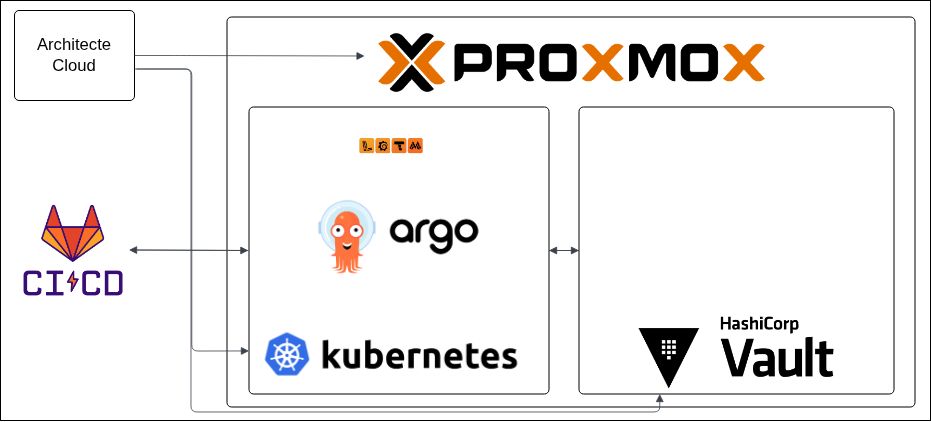
\includegraphics[width=0.9\textwidth]{figures/architecture-globale.png}
	\caption{Schéma d'architecture globale}
\end{figure}

\subsection{Infrastructure virtualisée et provisioning automatisé}

L'infrastructure physique est virtualisée au moyen d'une plateforme Proxmox. La création des ressources a été entièrement automatisée via une démarche Infrastructure as Code.

\subsubsection*{Infrastructure as Code avec Terraform}

Terraform a permis de décrire et de provisionner l'ensemble des ressources suivantes de façon déclarative et reproductible :
\begin{itemize}
	\item Les machines virtuelles dédiées aux nœuds Kubernetes (masters et workers) et aux services utilitaires.
	\item Les réseaux virtuels, sous-réseaux et interfaces.
	\item Les volumes de stockage attachés aux instances.
	\item Les configurations initiales via cloud-init.
\end{itemize}

Les modules Terraform ont été organisés par domaines fonctionnels afin de favoriser leur réutilisation et leur évolutivité.

\begin{figure}[H]
	\centering
	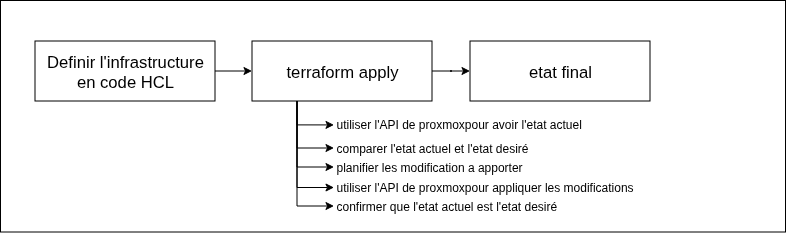
\includegraphics[width=0.8\textwidth]{figures/terraform-provisioning.png}
	\caption{Schéma du processus de provisioning automatisé avec Terraform}
\end{figure}

\subsubsection*{Configuration automatisée avec Ansible}

Après la création des ressources, Ansible assure la configuration des serveurs :
\begin{itemize}
	\item Installation et configuration du cluster Kubernetes.
	\item Déploiement des composants de monitoring et de sécurité.
	\item Configuration des services réseau et des paramètres système.
	\item Application des règles de sécurité renforcées.
\end{itemize}

Cette étape garantit l’homogénéité et la reproductibilité des environnements.

% Schéma Ansible configuration
\begin{figure}[H]
	\centering
	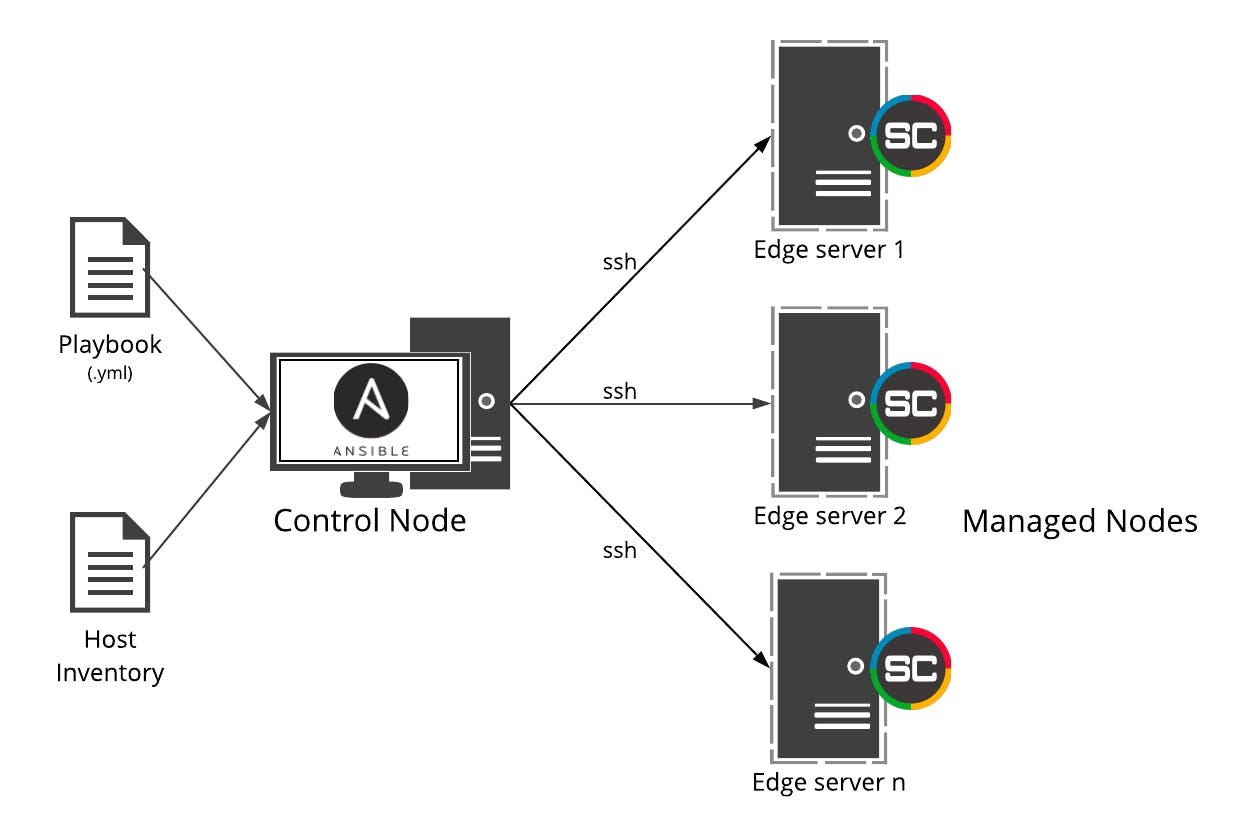
\includegraphics[width=0.8\textwidth]{figures/ansible-configuration.png}
	\caption{Processus d'automatisation de la configuration avec Ansible}
\end{figure}

\subsection{Orchestration et déploiement applicatif}

\subsubsection*{Cluster Kubernetes}

Kubernetes est le cœur de l’architecture d’orchestration. Il assure la gestion :
\begin{itemize}
	\item Du cycle de vie des conteneurs applicatifs.
	\item De l’équilibrage de charge et du scaling horizontal.
	\item De l’isolation des workloads.
\end{itemize}

\subsubsection*{Déploiement GitOps avec Argo CD}

Argo CD implémente une stratégie GitOps permettant :
\begin{itemize}
	\item Le déclenchement automatique des déploiements depuis un dépôt Git.
	\item La synchronisation continue des manifestes Kubernetes.
	\item La traçabilité complète des changements et la simplification des rollbacks.
\end{itemize}

\begin{figure}[H]
	\centering
	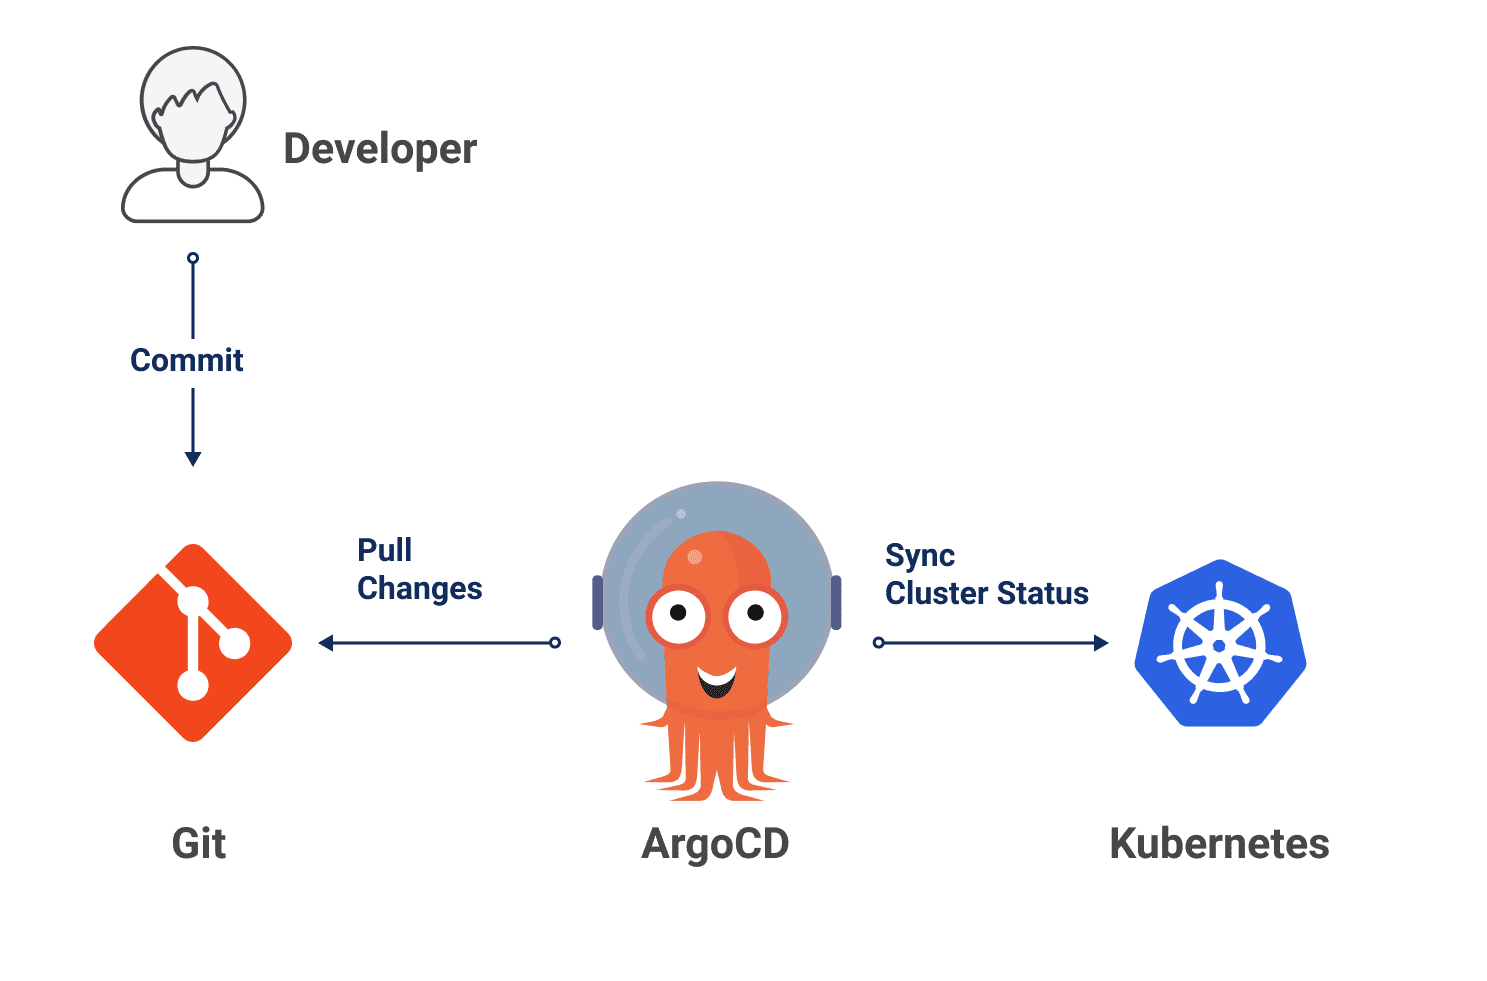
\includegraphics[width=0.9\textwidth]{figures/gitops-argo-cd.png}
	\caption{Flux GitOps des déploiements avec Argo CD}
\end{figure}

\subsection{Observabilité et monitoring}

La supervision s'appuie sur un ensemble d’outils intégrés :

\begin{itemize}
	\item \textbf{Prometheus} pour la collecte des métriques et des alertes.
	\item \textbf{Grafana} pour la visualisation des indicateurs.
	\item \textbf{Loki} pour la centralisation des logs applicatifs et système.
	\item \textbf{Tempo} pour la gestion des traces distribuées.
\end{itemize}

Cette stack assure une observabilité complète et un diagnostic précis en cas d’incident.

\begin{figure}[H]
	\centering
	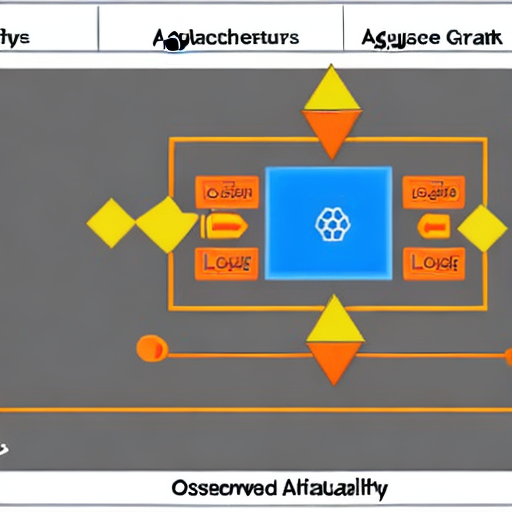
\includegraphics[width=0.85\textwidth]{figures/observabilite-stack.png}
	\caption{Architecture de la stack d'observabilité}
\end{figure}

\subsection{Stockage distribué et persistance des données}

Le stockage persistant est assuré par Longhorn, qui fournit :
\begin{itemize}
	\item Des volumes répliqués tolérants aux pannes.
	\item Des snapshots automatisés et des fonctionnalités de restauration.
	\item Une intégration transparente avec Kubernetes.
\end{itemize}

\subsection{Gestion sécurisée des secrets}

Vault joue le rôle de coffre-fort centralisé :
\begin{itemize}
	\item Stockage chiffré des mots de passe, certificats et tokens.
	\item Génération dynamique de secrets temporaires et rotation de secrets.
	\item Politiques d’accès granulaires pour limiter les droits.
\end{itemize}

\begin{figure}[H]
	\centering
	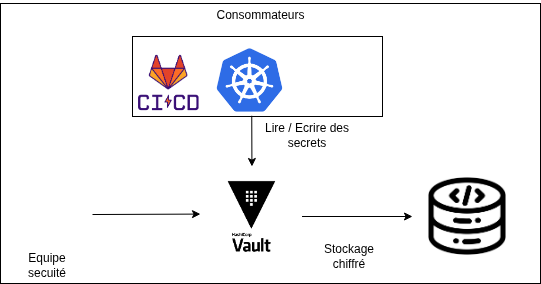
\includegraphics[width=0.8\textwidth]{figures/vault-gestion-secrets.png}
	\caption{Flux de gestion sécurisée des secrets avec Vault}
\end{figure}

\subsection{Sécurité réseau et accès administratifs}

La sécurité périmétrique est confiée à un pare-feu pfSense :
\begin{itemize}
	\item Contrôle des flux entrants et sortants via des règles spécifiques.
	\item Mise en place d’un VPN pour les accès administratifs.
	\item Surveillance active des connexions.
\end{itemize}

% Schéma pfSense
\begin{figure}[H]
	\centering
	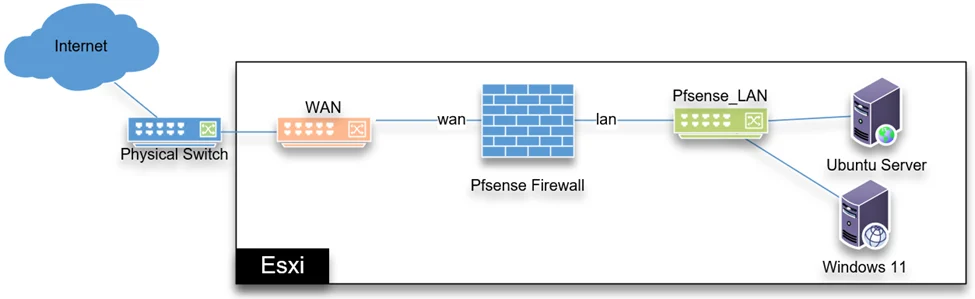
\includegraphics[width=0.85\textwidth]{figures/pfsense-securite.png}
	\caption{Architecture de sécurité réseau avec pfSense}
\end{figure}

\subsection{Services internes pour le cycle de vie applicatif}

Pour répondre aux besoins opérationnels des équipes, plusieurs services internes ont été déployés:
\begin{itemize}
	\item \textbf{GitLab} pour la gestion des dépôts, la CI/CD et la revue de code.
	\item \textbf{Harbor} comme registre privé de conteneurs.
	\item \textbf{YouTrack} pour le suivi des incidents et la gestion des tâches.
	\item \textbf{Nextcloud} pour le partage et l’archivage des documents.
\end{itemize}

Ces outils sont hébergés sur Kubernetes afin d’assurer leur haute disponibilité.

% Schéma services internes
\begin{figure}[H]
	\centering
	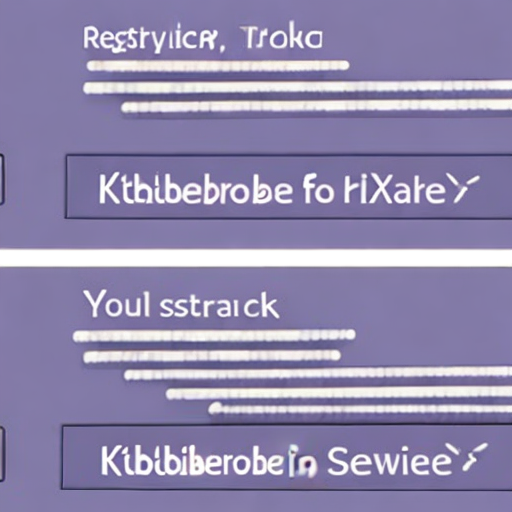
\includegraphics[width=0.85\textwidth]{figures/services-internes.png}
	\caption{Panorama des services internes}
\end{figure}

\subsection{Environnements de test et de production}

\begin{itemize}
	\item Des environnements de \textbf{test} et de \textbf{staging} reprenant la même architecture que la production ont été mis en place afin de valider les développements et les mises à jour.
	\item Les environnements de \textbf{production} ont été configurés avec des sauvegardes automatiques et des mesures renforcées de sécurité et de supervision.
\end{itemize}

\subsection{Intégration et automatisation des déploiements}

\textbf{GitLab CI/CD} joue un rôle central dans l'automatisation du cycle de vie applicatif. L’ensemble du pipeline est défini dans le fichier \texttt{.gitlab-ci.yml}, qui décrit les différentes étapes à exécuter pour chaque push, merge ou tag selon la configuration définie.

L’infrastructure GitLab repose sur plusieurs composants clés :
\begin{itemize}
	\item \textbf{\texttt{.gitlab-ci.yml}} : fichier principal décrivant les jobs et les stages du pipeline.
	\item \textbf{GitLab Runners} : exécutent les jobs dans des environnements isolés (VMs, containers...).
	\item \textbf{Variables GitLab} : utilisées pour stocker de manière sécurisée les credentials (tokens d’accès, clés API, identifiants, etc.), accessibles dans les jobs via des variables d’environnement.
	\item \textbf{Scripts et templates} : fichiers auxiliaires contenant les commandes d’automatisation (par exemple : \texttt{deploy.sh}, \texttt{test.sh}, \texttt{build.Dockerfile}).
\end{itemize}

\paragraph{Structure générale d’un pipeline GitLab CI}

Un pipeline CI/CD complet est généralement structuré autour des étapes suivantes :

\begin{itemize}
	\item \textbf{Validation}
	\item Formatage du code (ex : \texttt{black}, \texttt{prettier}, \texttt{clang-format}).
	\item Tests unitaires et fonctionnels (ex : \texttt{pytest}, \texttt{Jest}, \texttt{JUnit}).
	\item Analyse de dépendances (\texttt{OWASP Dependency-Check}, \texttt{safety}).
	\item Analyse de sécurité des secrets (\texttt{truffleHog}, \texttt{git-secrets}).
	\item Linting et analyse statique (ex : \texttt{ESLint}, \texttt{pylint}, \texttt{SonarQube}).
\end{itemize}

\begin{itemize}
	\item \textbf{Build}
	      \begin{itemize}
		      \item Compilation de binaires ou de librairies.
		      \item Construction d’images Docker avec \texttt{Dockerfile}.
		      \item Intégration des modules ou plugins nécessaires.
	      \end{itemize}

	\item \textbf{Package}
	      \begin{itemize}
		      \item Génération des artefacts (archives, packages, images).
		      \item Génération automatique de changelogs (\texttt{git-chglog}, \texttt{conventional-changelog}).
		      \item Mise à jour du \texttt{README}, documentation ou métadonnées.
	      \end{itemize}

	\item \textbf{Release}
	      \begin{itemize}
		      \item Création d’une release GitLab avec description, tag, et artefacts associés.
		      \item Publication vers des registries (DockerHub, GitLab Container Registry, PyPI, Maven, etc.).
		      \item Possibilité de signature cryptographique des artefacts.
	      \end{itemize}

	\item \textbf{Deploy}
	      \begin{itemize}
		      \item Déploiement automatique vers les environnements cibles (dev, staging, prod).
		      \item Utilisation de \texttt{kubectl}, \texttt{helm}, ou ArgoCD pour interagir avec Kubernetes.
		      \item Authentification via credentials sécurisés définis comme \texttt{CI/CD variables}.
	      \end{itemize}

	\item \textbf{Notify}
	      \begin{itemize}
		      \item Envoi de notifications Slack, Discord, Rocket.Chat, email ou webhook.
		      \item Génération de rapports HTML ou PDF avec les résultats des tests et des déploiements.
		      \item Archivage des logs dans des systèmes de monitoring (ELK, Loki, etc.).
	      \end{itemize}
\end{itemize}

\paragraph{Exemple de gestion des credentials}
Les variables sensibles telles que les clés d’accès API, tokens de déploiement ou credentials Kubernetes sont définies dans l’interface GitLab CI/CD (\texttt{Settings > CI/CD > Variables}) et injectées dans les jobs via :
\begin{verbatim}
deploy:
script:
- echo "$KUBECONFIG_SECRET" > kubeconfig
- kubectl --kubeconfig=kubeconfig apply -f k8s/
\end{verbatim}

\paragraph{Exemple de stage de release}
\begin{verbatim}
release:
stage: release
script:
- echo "Generating release..."
- git tag v${CI_COMMIT_SHORT_SHA}
- git push origin v${CI_COMMIT_SHORT_SHA}
- curl --header "PRIVATE-TOKEN: $GITLAB_TOKEN"
--data "name=Release v${CI_COMMIT_SHORT_SHA}&tag_name=v${CI_COMMIT_SHORT_SHA}"
"https://gitlab.com/api/v4/projects/${CI_PROJECT_ID}/releases"
\end{verbatim}

% Schéma GitLab CI
\begin{figure}[H]
	\centering
	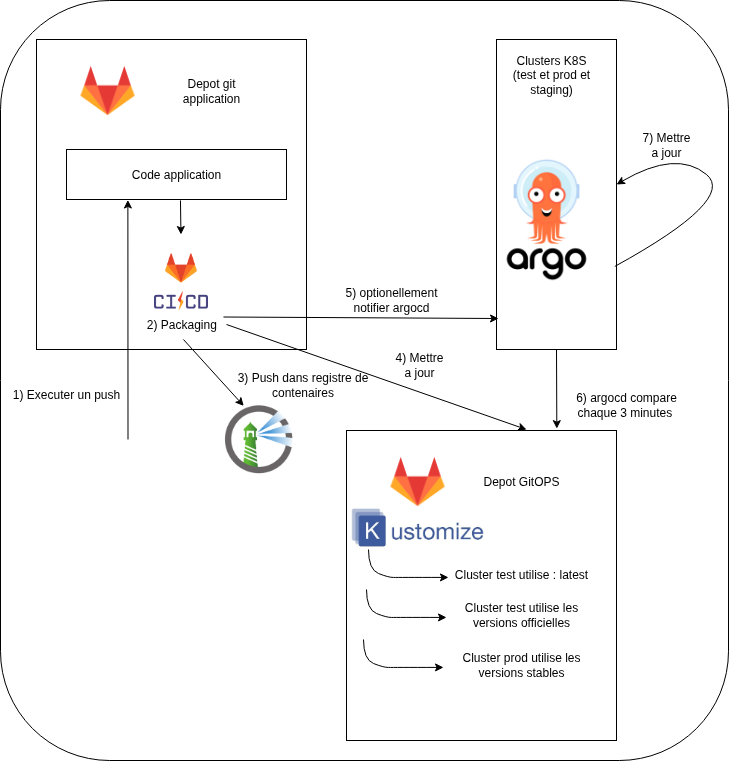
\includegraphics[width=0.85\textwidth]{figures/gitlab-ci.png}
	\caption{Processus d'intégration et de déploiement continu}
\end{figure}

\section{Fondements théoriques de l’automatisation des infrastructures}

\subsection{Évolution historique}

La gestion des systèmes d’information a connu une évolution rapide, marquée par plusieurs transformations majeures. Elle est passée de l’administration manuelle des serveurs physiques, où chaque déploiement nécessitait des opérations répétitives et susceptibles d’erreurs, à l’émergence des datacenters virtualisés et du Cloud Computing. Cette progression a été motivée par la recherche d’une meilleure agilité opérationnelle et par la nécessité de réduire les coûts d’exploitation.

La complexification des environnements informatiques a conduit à la formalisation de pratiques visant à automatiser la création, la configuration et la supervision des ressources. C’est dans ce contexte qu’a émergé le paradigme de l’Infrastructure as Code, qui constitue aujourd’hui un socle incontournable des démarches de modernisation.

\subsection{Approche DevOps}

Le développement des infrastructures modernes s’inscrit dans une démarche DevOps, qui associe les équipes de développement et d’exploitation dans une collaboration continue. Cette approche vise à réduire les cycles de livraison, améliorer la qualité logicielle et favoriser l’automatisation des processus. Elle s’appuie sur une culture de responsabilisation partagée, une intégration continue et une surveillance permanente des systèmes. DevOps contribue ainsi à faire converger les objectifs techniques et organisationnels, en alignant la production logicielle et les opérations.
\begin{figure} [H]
	\centering
	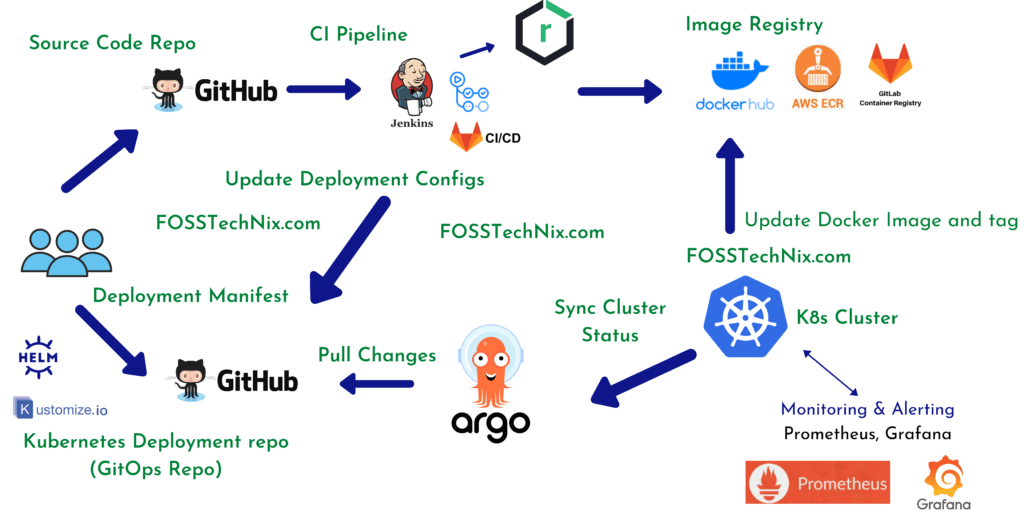
\includegraphics[width=.5\textwidth]{figures/Devops.png}
	\caption{Taches de DevOps}
	\label{fig:Taches de DevOps}
\end{figure}
\subsection{Modèles conceptuels}

L’Infrastructure as Code (IaC) désigne l’ensemble des méthodes et outils permettant de décrire l’état souhaité d’une infrastructure sous forme de fichiers de configuration versionnés et exécutables. Deux modèles se distinguent généralement : le modèle impératif, dans lequel l’utilisateur décrit la séquence exacte des opérations, et le modèle déclaratif, qui se concentre sur la définition de l’état final visé en laissant au moteur d’exécution la responsabilité d’y converger.

\subsection{Approche GitOps}

En prolongement de l’IaC, l’approche GitOps propose de faire du système de gestion de version la source unique de vérité pour la configuration et le déploiement applicatif. Elle se caractérise par un processus de déploiement automatisé, piloté par des agents qui observent l’état déclaré dans les dépôts et appliquent les modifications nécessaires aux environnements. Cette méthode garantit une traçabilité complète des évolutions, facilite le retour en arrière et renforce la cohérence entre les différents environnements. GitOps s’intègre naturellement avec les pipelines CI/CD, qui orchestrent la construction, les tests et la mise en production de façon systématique.

\section{Conteneurisation et orchestration}

\subsection{Principes de la conteneurisation}

La conteneurisation a constitué une rupture technologique majeure en introduisant une isolation légère des environnements d’exécution, en comparaison avec les machines virtuelles traditionnelles. Chaque conteneur encapsule l’application et ses dépendances, assurant ainsi une portabilité élevée et une reproductibilité des exécutions sur différents environnements.

Parmi les bénéfices les plus fréquemment identifiés figurent la réduction de la charge système, l’optimisation des coûts d’infrastructure, l’accélération des cycles de déploiement et une meilleure isolation des processus.

\subsection{Orchestration des conteneurs}

Pour coordonner ces conteneurs à grande échelle, des plateformes d’orchestration ont été développées. Kubernetes s’est progressivement imposé comme la solution de référence, grâce à sa capacité à automatiser le placement des workloads, l’ajustement dynamique des ressources, la relance des conteneurs défaillants et la gestion centralisée des configurations ainsi que des secrets. Ces fonctionnalités favorisent l’exploitation efficace d’environnements complexes et distribués.

\subsection{Patterns d’architecture cloud-native}

La conteneurisation et l’orchestration encouragent l’adoption de modèles applicatifs dits \emph{cloud-native}. Ces architectures reposent notamment sur le découpage en microservices, la scalabilité horizontale, la résilience par la redondance et le découplage entre l’infrastructure et les applications. Ces principes sont aujourd’hui largement adoptés par les entreprises souhaitant moderniser leurs systèmes d’information.

\section{Approches de supervision et d’observabilité}

\subsection{Enjeux de l’observabilité}

Dans des environnements distribués et dynamiques, l’observabilité est un facteur déterminant de fiabilité et de performance. Elle va au-delà de la supervision traditionnelle en visant une compréhension globale et en temps réel des comportements des systèmes. Cette démarche repose sur trois piliers essentiels : les métriques, qui mesurent l’état et les performances ; les logs, qui conservent l’historique des événements ; et les traces distribuées, qui permettent de suivre le parcours des requêtes au sein de l’architecture.

\subsection{Outils et standards de référence}

Différentes solutions se sont imposées comme standards de fait dans le domaine. Prometheus est souvent privilégié pour la collecte des métriques et la génération d’alertes, tandis que Grafana assure leur visualisation et leur suivi en temps réel. Elastic Stack ou Loki sont fréquemment utilisés pour l’agrégation et l’analyse des logs, et des outils tels que Jaeger et OpenTelemetry facilitent le traçage distribué. L’adoption de protocoles ouverts et d’API standardisées favorise leur intégration avec les plateformes d’orchestration.

\section{Sécurité des infrastructures automatisées}

\subsection{Principes de sécurité}

La sécurisation des infrastructures automatisées s’appuie sur le principe de \emph{Security by Design}, qui préconise l’intégration des mesures de protection dès les phases initiales de conception. Le modèle \emph{Zero Trust}, largement diffusé, repose notamment sur l’absence de confiance implicite accordée à un composant, l'identification, l’authentification et l’autorisation systématiques de chaque requête ainsi que la limitation des privilèges au strict nécessaire. Ces approches sont particulièrement adaptées aux environnements hybrides et multi-clouds.

\subsection{Gestion des secrets et des accès}

La gestion centralisée des secrets constitue une pratique essentielle pour sécuriser les identifiants, certificats et autres éléments sensibles. Elle repose sur le stockage chiffré, la rotation périodique des clés et la traçabilité des accès. Des outils spécialisés, tels que Vault, apportent des solutions robustes et éprouvées pour répondre à ces exigences.

\subsection{Sécurité périmétrique et segmentation}

La protection des infrastructures repose également sur des dispositifs périmétriques tels que les pare-feu, les listes de contrôle d’accès et la segmentation réseau. Ces mécanismes permettent de limiter la surface d’exposition, de cloisonner les environnements et de renforcer la résilience face aux attaques latérales. La mise en œuvre de politiques de filtrage strictes et le principe du moindre privilège complètent ces mesures pour réduire les risques d’intrusion.

\paragraph{Option : pfSense en tant que routeur et pare-feu principal}

Dans l’architecture retenue, il est possible de déployer pfSense comme machine virtuelle dédiée assurant le rôle de passerelle unique et de point de contrôle des flux réseau. Dans ce scénario, pfSense est connecté à deux interfaces réseau distinctes~:
\begin{itemize}
	\item Une interface \textbf{LAN}, reliée au réseau interne Proxmox et aux machines virtuelles.
	\item Une interface \textbf{WAN}, reliée au réseau externe (Internet).
\end{itemize}

Toutes les machines virtuelles définissent pfSense comme leur passerelle par défaut. Cela permet :
\begin{itemize}
	\item De centraliser le filtrage et le NAT.
	\item De contrôler et journaliser l’ensemble des flux entrants et sortants.
	\item D’appliquer des politiques de segmentation et de routage spécifiques par VLAN ou sous-réseau.
	\item D’établir des tunnels VPN (IPSec, OpenVPN) de manière centralisée.
\end{itemize}

Cette approche offre une séparation claire entre le plan de gestion (Proxmox) et le plan de données (trafic applicatif), améliorant la sécurité globale.

\begin{figure}[H]
	\centering
	\begin{tikzpicture}[
			node distance=2cm,
			box/.style={draw, rectangle, minimum width=3cm, minimum height=1cm, align=center},
			vm/.style={draw, rectangle, minimum width=2cm, minimum height=0.8cm, align=center}
		]

		% Nodes
		\node[box] (internet) {Internet};
		\node[box, below of=internet] (proxmox) {Proxmox Hyperviseur};
		\node[box, below of=proxmox] (pfsense) {VM pfSense \\ (Pare-feu / Routeur)};
		\node[box, below of=pfsense] (switch) {Réseau LAN Interne};
		\node[vm, left=1.5cm of switch] (vm1) {VM1};
		\node[vm, right=1.5cm of switch] (vm2) {VM2};

		% Arrows
		\draw[->] (internet) -- (proxmox);
		\draw[->] (proxmox) -- (pfsense);
		\draw[->] (pfsense) -- (switch);
		\draw[->] (switch) -- (vm1);
		\draw[->] (switch) -- (vm2);

	\end{tikzpicture}
	\caption{Architecture avec pfSense en tant que routeur et pare-feu principal}
	\label{fig:pfsense-router}
\end{figure}

Cette configuration permet de garantir que tout le trafic réseau transite par pfSense, offrant un contrôle périmétrique complet et la possibilité d’appliquer des politiques de sécurité avancées.
